%This is chapter 3
%%=========================================
\begingroup
\renewcommand{\cleardoublepage}{}
\renewcommand{\clearpage}{}
\chapter{Literature Review}
\section{Recognizing and Justifying Text Entailment through Distributional Navigation on Definition Graphs}
My work primarily builds on the work described in \cite{silva2018recognizing}. A detailed explanation follows in chapter \ref{chapter:description} as part of the project description.

\section{Red Opal: Product-Feature Scoring from Reviews}
In \cite{scaffidi2007red} the authors describe a system that is capable of extracting \textit{features} from reviews of products on online retailer platforms. The extracted features are ranked according to their own formula. The general idea is that features \textit{F} of products can only be nouns. The features F have to occur more often in all reviews of category \textit{C} than they do in written text of the language of the reviews. A more detailed explanation of how I use this work in my own follows in chapter \ref{chapter:description}.

\section{Effective Collaboration in Product Development via a
Common Sharable Ontology}
\label{section:share}
In \cite{mostefai2005effective} the authors describe how to build an ontology over products in a product development environment. They build an ontology that includes information about which specific parts a product contains to aid in the development of new products. As one of the goals of my work was to extend the already existing WordNet knowledge graph the parts of the paper describing the idea behind an ontology and how to build one were not very useful to this work.\\
The authors describe how they use the query mechanism of the Protégé \footnote{\url{https://protege.stanford.edu/}} platform for simple queries over their ontology. Indeed this works for very basic queries such as \textit{What are the design features of the “tee” part?} as used in the paper.\\
The authors give an example of a complex query but mention that it is not straightforward to perform. Furthermore their approach fails however for more complex queries or use cases, such as \textit{Which phones take the nicest pictures?} where there is no direct or obvious path to the target. In this particular case the knowledge of which part of a phone can take pictures (the camera) has to be connected to the act of \textit{taking a picture}. Using Protégé's query mechanism it is possible to find a connection between \textit{phone} and \textit{camera} but one has to know which feature can satisfy the user's request. The main difference between the query mechanism used by the authors and my approach is that the user does not need to have background knowledge to formulate the query in such a way that the system can work with it.

\section{Informed Recommender: Basing Recommendations on Consumer Product Reviews}
In \cite{aciar2007informed} the authors describe how they extract features from product reviews. They build an ontology of the products and how good or bad the customers think specific features (called \textit{concept} in the paper) for those products are. This ontology is then used in a recommender system\\
The difference to the feature extraction component used by me, based on \cite{scaffidi2007red}, is that the approach in this paper is based on machine learning. They train a classifier that labels sentences in the reviews into three categories: \textit{good}, for sentences that describe a feature that the reviewer thinks is good, \textit{bad} for sentences that describe a feature that the reviewer thinks is bad, and \textit{quality}, for sentences that describe the reviewers skill level. They use the "Rule Induction Kit for Text" (RIKTEXT) to extract rules for the three categories: \textit{fast} indicates a "good" text for example.
While the general idea is very similar to the Red Opal (\cite{scaffidi2007red}) system, the general approach is very different. To make use of their work, one has to create and label training data. The Red Opal approach only takes into account the frequency of the words and as such works without re-training or the need to create new training data to account for previously unknown features.\\
The labelled sentences are then the basis for the "concept extraction", which is comparable to the feature extraction in Red Opal. For their approach the authors manually extract the feature and define synonyms. The review sentences are then classified using the trained classifier and for each feature an entry in the ontology is created, showing how the reviewer likes specific product features.\\
The approach described here is not nearly as flexible as the Red Opal approach for feature extraction as it requires the creation of training data and creation of a synonym database which is very expensive. For this reason, I have used the Red Opal approach to extract both features and qualitative knowledge of the features from product reviews.

\chapter{Project Description}
\label{chapter:description}
\section{Crawler for product data}
To collect sufficient amounts of data for the feature extraction I have built a webcrawler using the Scrapy \footnote{\url{https://scrapy.org/}, accessed 2018-06-20} framework. The target was the \textit{drills} category on Amazon. 36375 reviews were crawled over the course of about 10 hours from 109 products.\\
The speed of crawling has to be slow, otherwise there is the risk of getting banned from Amazon \footnote{\url{https://doc.scrapy.org/en/latest/topics/practices.html\#avoiding-getting-banned}, accessed 2018-06-20}.\\
Due to the relatively slow speed and the limited number of products extracted during that time, I have looked for a different source of data to be able to build the feature extraction faster.\\
I have found a suitably large dataset of product reviews on Kaggle \footnote{\url{https://www.kaggle.com/PromptCloudHQ/amazon-reviews-unlocked-mobile-phones/data}, accessed 2018-06-20}. It includes 450212 total reviews over 4518 products in the \textit{phone} category.

\begin{table}[H]
\centering
\caption{Datasets overview}
\label{table:datasets}
    \begin{tabular}{l|l|l}
    Dataset & number of reviews & number of products \\ \hline
    Drills, using own crawler & 36375 & 109 \\ \hline
    Kaggle phone dataset  & 450212 & 4518 
    \end{tabular}
\end{table}

For my work I have used only the Kaggle dataset. Both the crawler I have built and the extracted reviews for products in the drills category are included in the code, see apendix \ref{chapter:code}.

\section{Feature extraction using Red Opal}
\label{sec:feature-extraction}
The core ideas of the feature extraction as discussed in \cite{scaffidi2007red} are the following:
\begin{itemize}
    \item a feature of a product can only be a noun
    \item the positions of the occurrences of a feature in a product review are irrelevant (bag-of-words assumption)
    \item the features discussed in the reviews occur more often than they do in other written or spoken text
\end{itemize}
The authors of the paper then develop a formula that can calculate the probability that a certain word occurs randomly the amount of times it does in all product reviews. The lower this probability, the higher the probability that it is a feature of the products. \\
The texts are processed using spaCy. It has good performance for POS-tagging which is the main component used in this work \footnote{\url{https://spacy.io/models/en#en_core_web_sm}, accessed 2018-06-20}. I use the Wikipedia frequency counts made available by the University of Leipzig \footnote{\url{http://wortschatz.uni-leipzig.de/en/download/}, accessed 2018-06-20} to have a frame of reference for the word frequency in written English as required by the Red Opal component.\\
Further I have made a major adjustment to the feature extraction: Only words that occur in the Wikipedia frequency corpus are considered. There are a lot of spelling errors in the reviews. Generally the algorithm of Red Opal is supposed to be resistant to them but in my experience this is not always the case when a lot of high scoring features are considered (the top 100 or even top 1000). As the goal is to extract features from products to extend an existing knowledge graph it makes sense to exclude words that are incorrectly spelled and thus not actually words. Another possibility would be to perform spelling correction on incorrectly spelled words but due to the time limitations of the seminar project this option was not explored.
Table \ref{table:scaff-features} shows the three highest scoring features and their score for the phone dataset.
\begin{minipage}{0.4\textwidth}
    \begin{table}[H]
    \vspace{-2em}
        \centering
        \caption{Highest scoring features}
        \label{table:scaff-features}
        \begin{tabular}{l|l}
            Feature & ln(P(feature)) \\ \hline
            phone & -15126199.8514816 \\
            screen & -1790234.63804627 \\
            battery & -1685233.74694203
        \end{tabular}
    \end{table}
\end{minipage}
\begin{minipage}{0.6\textwidth}
    \textit{Phone} is found because it is a noun and, as can be expected of reviews of phones, occurs very often and is thus the highest scoring feature by far. The others make sense as features of phones: Phones can have a screen and a battery.\\
    The feature extraction has been implemented from scratch based on the cited paper using Python 3.6 and the results are stored in a database using Django \footnotemark, a Python web framework with database support.
\end{minipage}
\footnotetext{\url{https://www.djangoproject.com/}}
\subsection{Insertion into WordnetGraph}
\label{subsec:insertion}
As currently the only extracted features come from phones, the only node in the original WordnetGraph is \textit{wnn:cellular\_telephone\_\_cellular\_phone\_\_cellphone\_\_cell\_\_mobile\_phone}.\\
A new RDF property is added, \textit{ns1:has\_feature} and triples in the known subject, predicate, object format added, where the object is one of the features found in the feature extraction. For the insertion into the existing graph rdflib \footnote{\url{http://rdflib.readthedocs.io/en/stable/}} was used. The idea of shaping the triples this way comes from \cite{silva2018categorization}.
\begin{table}[H]
\centering
\caption{RDF example}
\label{table:rdf-example}
\begin{tabular}{l|l|l}
Subject & Predicate & Object \\ \hline
wnn:cellular\_telephone\_\_cellular\_phone\_\_cellphone\_\_cell\_\_mobile\_phone & ns1:has\_feature & camera,\\
& & battery, \\
&  & screen...
\end{tabular}
\end{table}

\section{Product scoring}
\label{sec:product-scoring}
The found features (see section \ref{sec:feature-extraction}) are used to calculate so called \textit{Product Feature Scores}. They show how good a certain feature is given a specific product. This is used later to perform the product recommendation, refer to section \ref{sec:product-recommendation}.\\
\iffalse
The scores are calculated as defined in \cite{scaffidi2007red}:
\begin{align}
w(r, f) &= 2 - 2^{1 - o(r, f)} \text{ where \textit{r} is a review and \textit{f} is a feature contained in the review}\\
s(p, f) &= \frac{\sum_{r}w(r, f) * rating(r)}{\sum_{r}w(r, f)} \text{ where \textit{p} is a product and \textit{f} is a feature of the product}
\end{align}
\fi
I have added an additional score, based on the one that was defined in the paper.\\
\begin{minipage}{0.6\textwidth}
   \begin{align}
        \text{Let } l(p) &= \text{number of reviews of product p}\\
        m(p) &= 
        \begin{cases}
            1, \text{if } l(p) \text{ top 50\% \# reviews}\\
            0.75, \text{if } l(p) \text{ top 90\% \# reviews}\\
            0.5, \text{if } l(p) \text{ top 95\% \# reviews}\\
            0.25, \text{if } l(p) \text{ top 99\% \# reviews}\\
            0.1, \text{otherwise}
        \end{cases}\\
        mod\_s(p, f) &= m(p) * s(p, f)
    \end{align} 
\end{minipage}
\begin{minipage}{0.4\textwidth}
    \begin{table}[H]
    \centering
    \caption{Products ordered by number of reviews}
    \label{table:score-example}
    \begin{tabular}{l|l|l}
        Product & \# reviews & modifier \\ \hline
        A & 30 & 0.75\\
        B & 40 & 0.75\\
        C & 50 & 1
    \end{tabular}
    \end{table}
\end{minipage}

Product A has a modifier of 0.75 because it is not in the upper half of products in terms of number of reviews (the top 2), but it is in the top 90\% (top 3, 0.9 * 3 rounded up).\\
This means that the 1\% of reviews with the lowest number of reviews get a modifier of 0.1 and thus have their score lowered drastically. The idea behind this is to reward products that have a high number of reviews. A high number of reviews that assign a positive rating to a certain feature indicate that the score for this feature of this particular product is more meaningful or consistent than a product with only one review that assigns a positive rating to the same product.\\
As mentioned in the previous section \ref{sec:feature-extraction}, the extracted product feature scores are stored in the database.

\section{Implementation of graph navigation using WordnetGraph}
In this section I will outline how I have implemented the graph navigational algorithm as described in \cite{silva2018recognizing} and how the triples added in section \ref{sec:feature-extraction} play a role. For the sake of brevity the explanation of the original algorithm will be kept short and I will instead focus on the details of my implementation.\\
To find and justify textual entailment the algorithm attempts to find a path in the knowledge graph of the Wordnet definitions between two nodes, where nodes represent sets of synonyms, so called \textit{synsets}. The edges between the nodes come from the knowledge graph, and can be \textit{supertype} (apple has supertype fruit), \textit{has differentia quality} (oil furnace is a furnace with differentia quality 'burns oil'), \textit{has origin location} and others.\\
From the start node the algorithm finds all connected nodes and checks the semantic relatedness between the target node and the connected nodes. To calculate the semantic relatedness, I am using Indra \cite{indra2018}. Indra is a framework that can calculate word embeddings and semantic relatedness between pairs of words. A similar work is \cite{patwardhan2006using} but due to familiarity with Indra I have opted to use that. As the path between the source node and the target node is not known the semantic relatedness between pairs of nodes is used to measure the validity of an edge. If an edge leads to a node that has a low semantic relatedness with the target then most likely following this edge will not eventually lead to the target.\\
The next nodes to be visited come from the nodes with high enough relatedness' WordNet definitions. From those, the so called headwords are extracted (refer again to \cite{silva2018recognizing}). They are the most relevant words in the definition. I extract them using dependency parsing using the previously mentioned spaCy framework \footnote{\url{https://spacy.io}}.\\
Here I have made an experimental change to how the algorithm works: For supertype relations instead of extracting the main noun of the definition of the connected node I instead use the node itself as the next node.\\
An example:
\begin{itemize}
    \item \textit{apple} has supertype \textit{fruit}
    \item fruit has the definition: \textit{the ripened reproductive body of a seed plant}
    \item the extracted noun would be \textit{seed plant} or \textit{plant} and therefore the next node
    \item instead, I use \textit{fruit} as the next node
\end{itemize}
This change was made as a direct connection is the supertype relation indicates that all the properties and relations of the supertype node, the less specific node, apply to the subtype, the less specific node. In the example above, this would mean that all properties that hold for 'fruit' also hold for 'apple', as 'apple' is more specific than 'fruit', and all apples are fruit.\\
The currently visited node and the next possible nodes are concatenated and added to a stack. This represents the paths taken so far in the navigation. The algorithm continues from the last node in the path and continues as outlined until it reaches the target node. It terminates if a maximum number of paths between source and target is found or alternative if the maximum depth of the search is reached.
\subsection{Usage of product features in the graph}
\label{subsec:usage}
As I have mentioned in subsection \ref{subsec:insertion} I have added product features for phones into the graph. They added triples are considered in the navigational algorithm and open up new paths or shorten existing paths. Figure \ref{fig:cellphone-example} an example.\\
\begin{minipage}{0.5\textwidth}
    \begin{figure}[H]
        \centering
        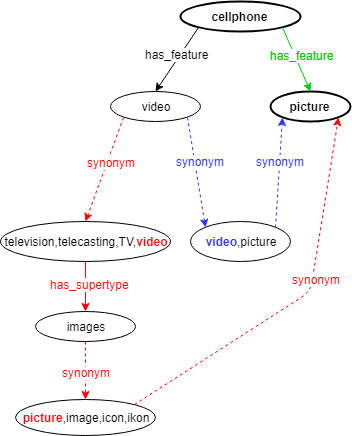
\includegraphics[scale=0.5]{fig/cellphone_navigation.png}
        \caption{Example of three paths found between 'cellphone' and 'picture'}
        \label{fig:cellphone-example}
    \end{figure}
\end{minipage}
\begin{minipage}{0.5\textwidth}
    The trivial case is the path $\text{cellphone} \rightarrow \text{picture}$. \textit{picture} was found as a feature of cellphones by the feature extraction (see section \ref{sec:feature-extraction}).\\
    A non-trivial case is the path $\text{cellphone} \rightarrow \text{video} \rightarrow \text{images} \rightarrow \text{picture}$. 
    \begin{itemize}
        \item \textit{video} was found as a feature of cellphones...
        \item  ... and is part of the synset \textit{television,telecasting,TV,video}...
        \item ... which has the supertype \textit{images} in the original knowledge graph...
        \item which is a synonym of \textit{picture}, the target node
    \end{itemize}
    The parameters for the navigational algorithm are as follows:
    \begin{itemize}
        \item Start node: cellphone.n
        \item End node: picture.n
        \item Minimum relatedness: 0.33
        \item Maximum number of paths: 3
        \item Maximum path depth: 6
    \end{itemize}
\end{minipage}

With the parameters specified my implementation of the navigational algorithm has found no path between \textit{cellphone} and \textit{picture}.
From the WordNet definition for \textit{cellphone}\footnote{WordNet: a hand-held mobile radiotelephone for use in an area divided into small sections, each with its own short-range transmitter/receive} it becomes clear that the trivial case of a direct connection is not possible regardless of implementation of the algorithm, as neither \textit{picture} or a synonym thereof appear in the definition. It can therefore be concluded that the extension of the knowledge graph with features extracted from product reviews is a valid approach that opens up new paths.

\subsection{Evaluation of the navigational graph algorithm}
To compare my implementation in Python with the original implementation I have used the BPI \footnote{\url{http://www.cs.utexas.edu/users/pclark/bpi-test-suite/}} dataset, as it is also used in the original paper. The metrics are taken directly from \cite{silva2018recognizing}.
\begin{table}[!htb]
    \begin{minipage}{.5\linewidth}
        \caption{Confusion matrix for BPI dataset}
        \label{table:bpi-eval}
        \begin{tabular}{llll}
             & Precision & Recall & F1 \\ \hline
            Original & 0.65  & 0.54 & 0.59  \\ \hline
            My system & 0.54 & 0.68 & 0.6 \\
        \end{tabular}
    \end{minipage}%
    \begin{minipage}{.5\linewidth}
        \centering
        \caption{Evaluation on BPI dataset}
        \label{table:bpi-matrix}
        \begin{tabular}{l|llll}
            & Yes &  & No &  \\ \hline
            Yes & 67 &  & 58 &  \\
            No & 31 &  & 93 & 
        \end{tabular}
    \end{minipage} 
\end{table}

The way textual entailment is checked is based on how it is described in the cited paper: Overlapping words for both text and hypothesis are removed and for the remaining set of words the k-highest scoring pairs (in terms of semantic relatedness, calculated using Indra) are kept and paths searched between them using the navigational algorithm. k is the maximum of the size of the two sets of non-overlapping words of text and hypothesis. Words with a low inverse document frequency (idf) are removed as well, as they can be reached from almost any node in the graph (see \cite{silva2018recognizing}).\\
I have added an additional restriction: I keep only verbs, nouns and proper nouns. Adjectives appear in the graph but only as the object in the triples and not as their own nodes with supertypes, differentia quality etc. To have a clear start and end they should either be verbs or nouns as both of them appear as \textit{WordNetNounSynset} and \textit{WordNetVerbSynset} in the graph, respectively, with supertypes and properties.\\
Because of this added limitation some of the pairs used for the evaluation do not have pairs of words that can be used for the algorithm. Those pairs are then considered to have no entailment. The confusion matrix with those empty pairs excluded from the evaluation can be seen in table \ref{table:bpi-matrix-non-empty}.

\begin{table}[!htb]
    \begin{minipage}{.5\linewidth}
        \caption{Confusion matrix, BPI\\ dataset without empty pairs}
        \label{table:bpi-matrix-non-empty}
        \begin{tabular}{llll}
             & Precision & Recall & F1 \\ \hline
             & 0.71 & 0.68 & 0.7 \\
        \end{tabular}
    \end{minipage}%
    \begin{minipage}{.5\linewidth}
        \centering
        \caption{Evaluation BPI\\ dataset without empty pairs}
        \label{table:bpi-eval-non-empty}
        \begin{tabular}{l|llll}
            & Yes &  & No &  \\ \hline
            Yes & 67 &  & \textcolor{red}{27} &  \\
            No & 31 &  & \textcolor{red}{28} & 
        \end{tabular}
    \end{minipage} 
\end{table}
21 text-hypothesis pairs with entailment were unable to be checked due to not having pairs of words after removing overlapping words and keeping only nouns and verbs. Meanwhile 71 pairs without entailment were excluded. This indicates that my restriction of keeping only nouns and verbs in addition to the other restrictions might be valid as significantly more pairs without textual entailment were excluded than pairs with textual entailment. The metrics for this confusion matrix can be seen in table \ref{table:bpi-eval-non-empty}.
The metrics improve by a significant amount. One way this could be used is to use the navigational algorithm to check for textual entailment if there are pairs of words that the algorithm can use and to use a different method for those text-hypothesis pairs where too many words are filtered out.

\subsection{Product recommendation}
\label{sec:product-recommendation}
As an example of how textual entailment in conjunction with product feature scores can be used in a real system I have built a simple product recommender. One example query is \textit{Which cellphones take the nicest pictures?}.\\
I have analysed a few possible queries for product recommendation and also taken into account the queries mentioned in \cite{mostefai2005effective} (see section \ref{section:share}). By doing this, I have noticed that the two main ways queries are formulated are those that focus on an action, such as \textit{charging} in the case of phones, and those that focus on a noun, such as \textit{pictures} or \textit{apps}.\\
Using the dependency parsing of spaCy I have analysed those two types of queries to extract suitable word pairs for use in the navigational algorithm. Figure \ref{fig:dep-example} shows an example parse tree.
\begin{figure}[H]
    \centering
    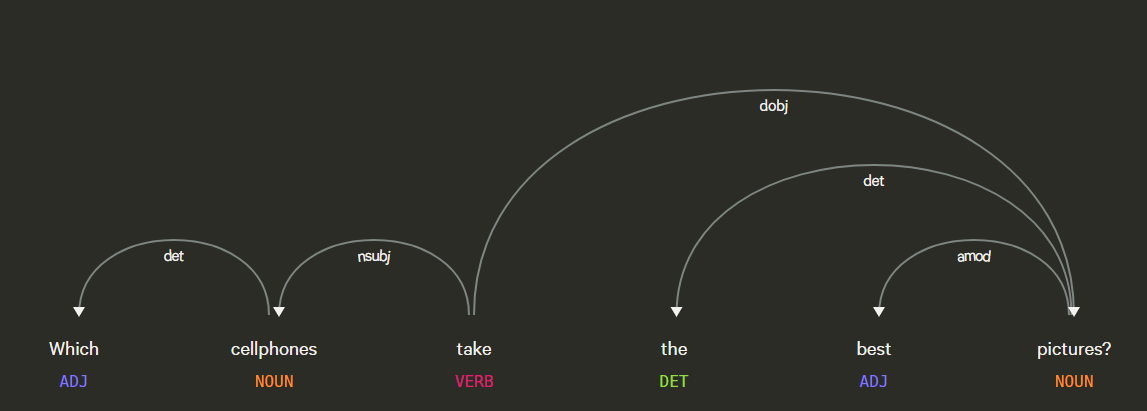
\includegraphics[scale=0.5]{fig/dep-example.PNG}
    \caption{Parse tree example using \url{https://explosion.ai/demos/displacy}}
    \label{fig:dep-example}
\end{figure}

Based on the analysis using dependency parsing, I make the following assumptions about the queries:
\begin{itemize}
    \item the \textit{NSUBJ} is always the category of product
    \item if the \textit{DOBJ} is a noun then that is the target feature
    \item if the \textit{DOBJ} is not a noun then the \textit{ROOT} is the target and always a verb
\end{itemize}
I consider the problem of finding features that match the query to be a textual entailment problem. The query and the product features can be transformed into text and hypothesis pairs like so:
\begin{itemize}
    \item Text: A \textit{PRODUCT-CATEGORY} has feature \textit{SOME-FEATURE}.
    \item Hypothesis: A \textit{PRODUCT-CATEGORY} can \textit{TARGET-VERB}.
    \item Hypothesis: A \textit{PRODUCT-CATEGORY} has \textit{TARGET-NOUN}.
\end{itemize}
Using the example from figure \ref{fig:dep-example}, this would become:
\begin{itemize}
    \item Text: A \textit{cellphone} has feature \textit{camera}.
    \item Hypothesis: A \textit{cellphone} has \textit{picture}.
\end{itemize}

Neither text nor hypothesis are explicitly created like this, but the idea behind this brought me to my current implementation. I search for paths between the category of the query (phone) and the target (target verb or target noun) and collect all paths that I find. Since the product features were added to the knowledge graph and as has been shown in \ref{subsec:usage} they can be used to find new path it makes sense to search for a path from the product category and the target feature. It is possible that there is a path that does not make use of the product features, but this case implies that none of the products in that category have the features that were used in that path.\\
I keep all the paths that have a \textit{has\_feature} relation in them: Those features are the ones that are relevant to the query. Once the features that match the query are extracted, showing products that have those features and their scores as calculated in \ref{sec:product-scoring} is simple. The data is stored in the database and the matching products simply have to be retrieved. Figure \ref{fig:query-example} shows an example query. The tabs are matching features that were found and one example path from start node to end node is shown, together with matching products and information about their scores for that particular feature.

\begin{figure}[H]
    \centering
    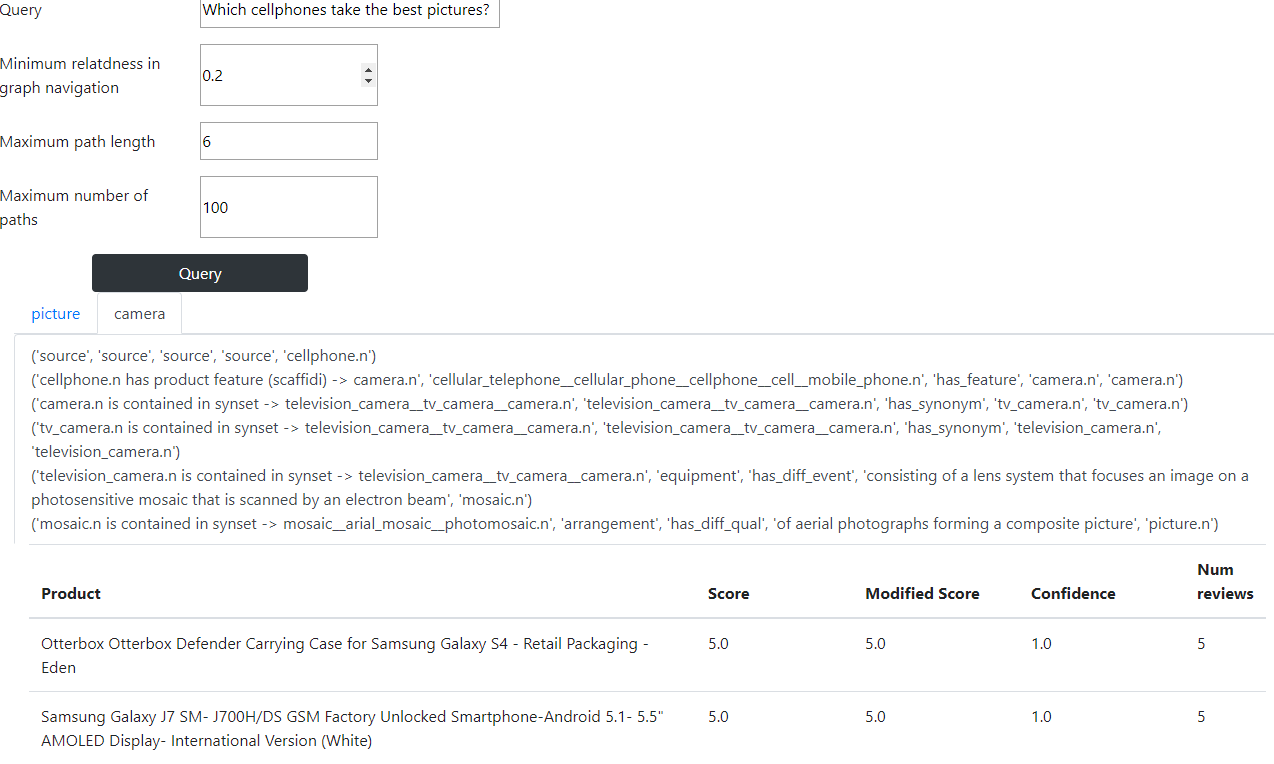
\includegraphics[scale=0.5]{fig/query-example.PNG}
    \caption{Example query and result}
    \label{fig:query-example}
\end{figure}


\chapter{Summary}

\section{Discussion and recommendations for further work}
The developed system is meant to be a proof-of-concept of augmenting an existing knowledge
graph with knowledge about product categories based on features of those products extracted
from product reviews. The biggest issue is that my implementation has a lower precision when
performing an evaluation than the original implementation (see 3.5). The problem here is most
likely an error in the implementation but nonetheless when excluding the entailment pairs from
the evaluation that do not produce checkable word pairs the results of the system are quite
robust (see \ref{table:bpi-eval-non-empty}).
As the product recommendation is very basic right now it is a good basis for an extension of my
work. One option is to explicitly create entailment pairs from the extracted product
features as mentioned in section \ref{sec:product-recommendation} and find all product features that match the query first
instead of looking for paths between the category and the target of the query.


\section{Summary}
As part of this seminar I have extended the existing WordNet knowledge graph based on \cite{silva2018recognizing} with features extracted from product reviews using an approach by \cite{scaffidi2007red}. As a
proof-of-concept features were extracted from 450212 reviews of products in the cellphone category
on Amazon and new triples added to the knowledge graph to augment the navigational
algorithm with new paths. I have shown that this is a valid approach by showcasing entirely new
paths in the graph in section \ref{subsec:usage}.
Furthermore I have built a basic product recommender that makes use of the graph navigational
algorithm to perform basic product recommendation based on user queries.


\endgroup